% !TeX program = xelatex
\documentclass[a4paper,10pt]{article}

% ============================================================================
% សន្លឹកកិច្ចការសិស្សបំពេញចន្លោះ ស-ខ្មៅ និងប្លង់ក្ដារខៀន/ចម្លើយគ្រូ (គ្មាន LCD / គ្មានកន្ត្រៃ)
% មេរៀនទី២ (១.២ និង ២.)៖ លក្ខណៈចែកដាច់ផលបូកដក និងតួចែកពហុគុណ — ត្រូវគ្នា ១០០% នឹង LS_Plan_DIV22.tex
% ============================================================================
\usepackage[a4paper, left=1.0cm, right=1.0cm, top=0.75cm, bottom=1.00cm, footskip=0.52cm]{geometry}
\usepackage{amsmath}
\usepackage{unicode-math}
\usepackage{fontspec}
\usepackage{array, colortbl}
\usepackage[table]{xcolor}
\usepackage{enumitem}
\usepackage{pifont}
\usepackage{fancyhdr}
\usepackage{lastpage}
\usepackage{tikz}
\usepackage[most]{tcolorbox}
\usetikzlibrary{calc, arrows.meta, decorations.pathreplacing, positioning, babel}

\makeatletter
\let\@expl@@@mark@update@singlecol@structures@@\relax
\makeatother

\providecommand{\NGSFindFonts}{%
  \IfFileExists{C:/Windows/Fonts/cambria.ttc}{%
    \def\NGSSysPath{C:/Windows/Fonts/}%
    \def\NGSUserPath{C:/Users/KIT/AppData/Local/Microsoft/Windows/Fonts/}%
  }{%
    \IfFileExists{./fonts/KhmerOSsiemreap.ttf}{\def\NGSSysPath{./fonts/}\def\NGSUserPath{./fonts/}}{%
    \IfFileExists{../fonts/KhmerOSsiemreap.ttf}{\def\NGSSysPath{../fonts/}\def\NGSUserPath{../fonts/}}{%
    \IfFileExists{../../fonts/KhmerOSsiemreap.ttf}{\def\NGSSysPath{../../fonts/}\def\NGSUserPath{../../fonts/}}{%
    \IfFileExists{../../../fonts/KhmerOSsiemreap.ttf}{\def\NGSSysPath{../../../fonts/}\def\NGSUserPath{../../../fonts/}}{%
    \IfFileExists{../../../../fonts/KhmerOSsiemreap.ttf}{\def\NGSSysPath{../../../../fonts/}\def\NGSUserPath{../../../../fonts/}}{%
    \IfFileExists{../../../../../fonts/KhmerOSsiemreap.ttf}{\def\NGSSysPath{../../../../../fonts/}\def\NGSUserPath{../../../../../fonts/}}{%
    \IfFileExists{../../../../../../fonts/KhmerOSsiemreap.ttf}{\def\NGSSysPath{../../../../../../fonts/}\def\NGSUserPath{../../../../../../fonts/}}{%
      \def\NGSSysPath{../../../../../../../fonts/}\def\NGSUserPath{../../../../../../../fonts/}%
    }}}}}}}%
  }%
}
\NGSFindFonts

\setmathfont[Path={\NGSSysPath}, FontIndex=1, Scale=1.02]{cambria.ttc}
\defaultfontfeatures{Ligatures=TeX}

\setmainfont[
  Path={\NGSUserPath}, Extension=.ttf, Script=Khmer,
  BoldFont={KhmerOSsiemreap}, BoldFeatures={FakeBold=1.8},
  ItalicFont={KhmerOSsiemreap}, ItalicFeatures={FakeSlant=0.25},
  BoldItalicFont={KhmerOSsiemreap}, BoldItalicFeatures={FakeBold=1.8, FakeSlant=0.25}
]{KhmerOSsiemreap}

\newfontfamily\muol[Path={\NGSUserPath}, Extension=.ttf, Script=Khmer]{KhmerOSmuollight}
\newfontfamily\TimesEn[Path={\NGSSysPath}, Extension=.ttf, BoldFont={timesbd}, ItalicFont={timesi}, BoldItalicFont={timesbi}]{times}
\newfontfamily\CalibriFont[Path={\NGSSysPath}, Extension=.ttf]{calibri}

\XeTeXlinebreaklocale "km"
\XeTeXlinebreakskip = 0pt plus 1pt minus 0.1pt

\definecolor{panelgray}{gray}{0.94}
\definecolor{headgray}{gray}{0.85}

\pagestyle{fancy}
\fancyhf{}
\renewcommand{\headrulewidth}{0pt}
\fancyfoot[L]{\fontsize{7.4pt}{9.5pt}\selectfont អនុវិទ្យាល័យព្រះក្រសាំង \en{|} គ្រូ៖ ហុក ប៊ុនថែន \en{|} មេរៀនទី២ (១.២ និង ២.) ផលបូកដកចែកដាច់ និងតួចែកពហុគុណ \en{|} ថ្ងៃសុក្រ ទី១៣ ខែវិច្ឆិកា ឆ្នាំ២០២៦}
\fancyfoot[R]{\fontsize{7.8pt}{10pt}\selectfont ទំព័រ \en{\thepage\ / \pageref{LastPage}}}

\setlength{\parindent}{0pt}
\setlength{\parskip}{0pt}
\setlength{\tabcolsep}{4pt}
\newcolumntype{L}[1]{>{\raggedright\arraybackslash}p{#1}}
\newcolumntype{C}[1]{>{\centering\arraybackslash}p{#1}}

\newcommand{\en}[1]{{\TimesEn #1}}
\newcommand{\enbf}[1]{{\TimesEn\bfseries #1}}
\newcommand{\unit}[1]{\,\text{\en{#1}}}
\newcommand{\cnum}[1]{\mbox{\fontsize{10pt}{12pt}\selectfont\ding{\numexpr181+#1\relax}}}
\newcommand{\chkbox}{\tikz[baseline=-0.15ex]\draw[black, line width=0.85pt, fill=white] (0,0) rectangle (0.24cm,0.24cm);}
\newcommand{\ansbox}[1][1.75cm]{\,\tikz[baseline=-0.65ex]\draw[black, line width=0.65pt, fill=white] (0,0) rectangle (#1, 0.42cm);\,}
\newcommand{\dbox}{\,\tikz[baseline=-0.35ex]\draw[black, line width=0.75pt, fill=white] (0,0) rectangle (0.38cm,0.38cm);\,}
\newcommand{\dotline}[1][2.2cm]{\makebox[#1]{\dotfill}}

\newcommand{\pagebanner}[2]{%
  \begin{tcolorbox}[
    enhanced, sharp corners, colback=headgray, colframe=black,
    boxrule=1.05pt, boxsep=1pt, top=2.5pt, bottom=2.5pt, left=6pt, right=6pt,
    after skip=3.5pt
  ]
    {\muol\fontsize{9.0pt}{13.2pt}\selectfont #1}\hfill{\fontsize{8.0pt}{11.2pt}\selectfont\textbf{#2}}
  \end{tcolorbox}%
}

\newcommand{\secstrip}[2]{%
  \vspace{3pt}%
  \begin{tcolorbox}[
    enhanced, sharp corners, colback=panelgray, colframe=black,
    boxrule=0.8pt, boxsep=0.8pt, top=2pt, bottom=2pt, left=5pt, right=5pt,
    after skip=3pt
  ]
    {\muol\fontsize{8.5pt}{12.2pt}\selectfont #1}\hfill{\fontsize{7.8pt}{10.8pt}\selectfont\textit{#2}}
  \end{tcolorbox}%
}

\begin{document}
\fontsize{9.5pt}{14.5pt}\selectfont

% ============================================================================
% ទំព័រទី ១៖ សន្លឹកកិច្ចការសិស្ស (ផ្នែកមុខ៖ E1 -> E2 -> E3)
% ============================================================================
\pagebanner{សន្លឹកកិច្ចការសិស្ស \enbf{(}១\enbf{.}២ ផលបូកដកចែកដាច់ និង ២\enbf{.} តួចែកពហុគុណ\enbf{)} \enbf{--} ផ្នែកមុខ}{ថ្នាក់ទី៧ \en{|} សៀវភៅគោល ទំ.១៨--១៩}

\begin{tcolorbox}[
  enhanced, sharp corners, colback=white, colframe=black,
  boxrule=0.8pt, boxsep=1.5pt, top=3.5pt, bottom=3.5pt, left=5pt, right=5pt,
  after skip=4pt
]
  \fontsize{9.0pt}{13.0pt}\selectfont
  \textbf{ឈ្មោះសិស្ស៖} \dotline[4.3cm] \quad
  \textbf{សមាជិកក្រុម៖} \dotline[4.3cm] \quad
  \textbf{ថ្នាក់ទី៖} ៧\dotline[0.9cm] \quad
  \textbf{ក្រុមទី៖} \dotline[1.0cm]
\end{tcolorbox}

% --- E1 Engage ---
\secstrip{ផ្នែកទី ១ \enbf{(E1 - Engage)} ៖ បេសកកម្មអន្ទាក់ពាក្យ «តួចែក» និង «ពហុគុណ»}{រយៈពេល ៣ នាទី (គូស \ding{51} ក្នុង \chkbox)}

\begin{tcolorbox}[
  enhanced, sharp corners, colback=white, colframe=black,
  boxrule=0.8pt, boxsep=2pt, top=4pt, bottom=4pt, left=6pt, right=6pt
]
  គេមានសមភាព $18 = 3 \times 6$ (ពោលគឺ $18 \div 6 = 3$ ចែកដាច់គ្មានសំណល់)៖\\[2.5pt]
  $\bullet$ \chkbox\ \textbf{សិស្ស ក៖} «លេខ $18$ ហៅថា\textbf{តួចែក}នៃ $6$ ហើយលេខ $6$ ហៅថា\textbf{ពហុគុណ}នៃ $18$»\\[2pt]
  $\bullet$ \chkbox\ \textbf{សិស្ស ខ៖} «លេខ $6$ ហៅថា\textbf{តួចែក}នៃ $18$ ហើយលេខ $18$ ហៅថា\textbf{ពហុគុណ}នៃ $6$!»
\end{tcolorbox}

\vfill

% --- E2 Explore ---
\secstrip{ផ្នែកទី ២ \enbf{(E2 - Explore)} ៖ ផលបូកដកចែកដាច់ និងគូកត្តាឥន្ទធនូ (ទំ.១៨--១៩)}{រយៈពេល ១១ នាទី}

\textbf{សកម្មភាព ១ (\en{E2-A} — ៤.៥ នាទី)៖ ១.២ លក្ខណៈចែកដាច់នៃផលបូកនិងផលដក (ឧទាហរណ៍ ទំ.១៨)}

\begin{tcolorbox}[
  enhanced, sharp corners, colback=white, colframe=black,
  boxrule=0.8pt, boxsep=2.5pt, top=4pt, bottom=4pt, left=6pt, right=6pt
]
  គេមាន $512$ ចែកដាច់នឹង $2$ និង $326$ ចែកដាច់នឹង $2$៖\\[3pt]
  $\bullet$ \textbf{១) ផលបូក៖} $512 + 326 =$ \ansbox[1.6cm] $\to$ តើចែកដាច់នឹង $2$ ដែរឬទេ? \dotline[1.6cm] (ព្រោះខ្ទង់រាយជាលេខ \dotline[0.8cm])\\[3pt]
  $\bullet$ \textbf{២) ផលដក៖} $512 - 326 =$ \ansbox[1.6cm] $\to$ តើចែកដាច់នឹង $2$ ដែរឬទេ? \dotline[1.6cm] (ព្រោះខ្ទង់រាយជាលេខ \dotline[0.8cm])
\end{tcolorbox}

\vspace{4pt}
\textbf{សកម្មភាព ២ (\en{E2-B} — ៦.៥ នាទី)៖ ២. តួចែកនិងពហុគុណតាមគូកត្តាឥន្ទធនូ (ឧទាហរណ៍ ១ និង ២ ទំ.១៨)}

\begin{tcolorbox}[
  enhanced, sharp corners, colback=white, colframe=black,
  boxrule=0.8pt, boxsep=2.5pt, top=4pt, bottom=4pt, left=6pt, right=6pt
]
  $\bullet$ \textbf{១) រកតួចែកនៃ $18$៖} $18 = 1\times$ \dotline[0.9cm] $= 2\times$ \dotline[0.9cm] $= 3\times$ \dotline[0.9cm]\\[2.5pt]
  \hspace*{0.3cm}ដូចនេះ តួចែកទាំងអស់នៃ $18$ មាន $6$ ចំនួនគឺ៖ $1,\ 2,\ 3,$ \dotline[0.9cm], \dotline[0.9cm] និង \dotline[0.9cm] ហើយ $18$ ជា\textbf{ពហុគុណ}នៃចំនួនទាំងនេះ ។\\[3pt]
  \begin{center}
  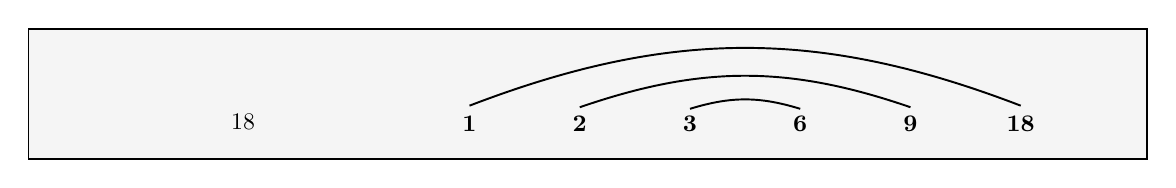
\begin{tikzpicture}[x=1cm, y=1cm, every node/.style={font=\fontsize{8.6pt}{11.5pt}\selectfont, text=black}]
    \draw[black, line width=0.65pt, fill=gray!8] (0,0) rectangle (14.2,1.65);
    \node[anchor=west] at (0.3,0.48) {\textbf{គំរូធ្នូគូកត្តាឥន្ទធនូនៃ $18$៖}};
    \node at (5.6,0.45) {$\mathbf{1}$};
    \node at (7.0,0.45) {$\mathbf{2}$};
    \node at (8.4,0.45) {$\mathbf{3}$};
    \node at (9.8,0.45) {$\mathbf{6}$};
    \node at (11.2,0.45) {$\mathbf{9}$};
    \node at (12.6,0.45) {$\mathbf{18}$};
    \draw[black, line width=0.7pt] (5.6,0.68) to[bend left=21] (12.6,0.68);
    \draw[black, line width=0.7pt] (7.0,0.66) to[bend left=19] (11.2,0.66);
    \draw[black, line width=0.7pt] (8.4,0.64) to[bend left=17] (9.8,0.64);
  \end{tikzpicture}
  \end{center}
  $\bullet$ \textbf{២) រកតួចែកនៃ $100$ តាមគូកត្តា៖} $100 = 1\times 100 = 2\times$ \dotline[0.9cm] $= 4\times$ \dotline[0.9cm] $= 5\times$ \dotline[0.9cm] $= 10\times$ \dotline[0.9cm]\\[2.5pt]
  \hspace*{0.3cm}ដូចនេះ តួចែកទាំងអស់នៃ $100$ គឺ៖ $1,\ 2,\ 4,\ 5,\ 10,$ \dotline[0.9cm], \dotline[0.9cm], \dotline[0.9cm] និង \dotline[1.0cm] ($9$ ចំនួន) ។\\[3pt]
  $\bullet$ \textbf{៣) ឧទាហរណ៍ ៣ (ទំ.១៨) — រកពហុគុណ ៥ ដំបូងនៃ $7$៖} $7\times 1 = 7,\ 7\times 2 =$ \dotline[0.9cm], $7\times 3 =$ \dotline[0.9cm], $7\times 4 =$ \dotline[0.9cm], $7\times 5 =$ \dotline[0.9cm], $\dots$
\end{tcolorbox}

\vfill

% --- E3 Explain ---
\secstrip{ផ្នែកទី ៣ \enbf{(E3 - Explain)} ៖ វិធានទូទៅ និងធនាគារហេតុផល \enbf{B\&W}}{រយៈពេល ៦ នាទី}

\begin{tcolorbox}[
  enhanced, sharp corners, colback=white, colframe=black,
  boxrule=0.85pt, boxsep=2.5pt, top=4pt, bottom=4pt, left=6pt, right=6pt
]
  ១) បើតួនីមួយៗនៃផលបូក ឬផលដក ចែកដាច់នឹងចំនួនតែមួយដូចគ្នា នោះ \dotline[2.8cm] របស់វា ក៏ចែកដាច់នឹងចំនួននោះដែរ ។\\[2.5pt]
  ២) គ្រប់ចំនួនគត់ $n$ មានតួចែក \dotline[0.8cm] និង \dotline[1.3cm] ជានិច្ច ។ បើ $a$ ចែកដាច់នឹង $b$ នោះ $b$ ជា\dotline[1.4cm]នៃ $a$ ហើយ $a$ ជា\dotline[1.5cm]នៃ $b$ ។\\[2.5pt]
  ៣) \textbf{សម្គាល់ (ទំ.១៨)៖} ចំនួនតួចែកនៃ $n$ មាន \dotline[1.8cm] ($\le n$) រីឯពហុគុណនៃ $n$ មាន \dotline[2.6cm] ។\\[3.5pt]
  \tikz\draw[black, dashed, line width=0.5pt] (0,0) -- (18.4cm,0);\\[3pt]
  \fontsize{8.7pt}{12.8pt}\selectfont
  \textbf{ធនាគារហេតុផល (\en{Warrant Bank})៖} \quad
  \cnum{1} $(a\div k,\ b\div k) \implies (a\pm b)\div k$ \quad
  \cnum{2} តួចែកនៃ $n$ ($\le n$, រួមទាំង $1$ និង $n$)\\
  \cnum{3} ពហុគុណនៃ $b$ ($a = b\times q$, រាប់មិនអស់) \quad
  \cnum{4} គូកត្តាឥន្ទធនូ (ផ្គូផ្គងពីក្រៅចូលក្នុងកុំឱ្យបាត់តួចែក)
\end{tcolorbox}

% ============================================================================
% ទំព័រទី ២៖ សន្លឹកកិច្ចការសិស្ស (ផ្នែកខាងខ្នង៖ E4 -> E5 -> កិច្ចការផ្ទះ)
% ============================================================================
\clearpage
\pagebanner{សន្លឹកកិច្ចការសិស្ស \enbf{(}១\enbf{.}២ ផលបូកដកចែកដាច់ និង ២\enbf{.} តួចែកពហុគុណ\enbf{)} \enbf{--} ផ្នែកខាងខ្នង}{ថ្នាក់ទី៧ \en{|} សៀវភៅគោល ទំ.១៨--១៩, ២៤}

% --- E4 Elaborate ---
\secstrip{ផ្នែកទី ៤ \enbf{(E4 - Elaborate)} ៖ លំហាត់គំរូតាមសៀវភៅគោល ទំ.១៨--១៩}{រយៈពេល ១០ នាទី}

\begin{tcolorbox}[
  enhanced, sharp corners, colback=white, colframe=black,
  boxrule=0.8pt, boxsep=2.5pt, top=4.5pt, bottom=4.5pt, left=6pt, right=6pt
]
  $\bullet$ \textbf{១) គំរូ ១.២ (ទំ.១៨)៖} គេមានបីចំនួនគត់តគ្នាគឺ $a,\ a+1,\ a+2$ ($a$ ជាចំនួនគត់) ។ បង្ហាញថាផលបូកចំនួនទាំងបីចែកដាច់នឹង $3$៖\\[3pt]
  \hspace*{0.3cm}គេបាន $a + (a+1) + (a+2) =$ \ansbox[2.4cm] ។ ដោយ $3a$ ចែកដាច់នឹង \dotline[0.9cm] ហើយ $3$ ចែកដាច់នឹង \dotline[0.9cm] នោះផលបូកចែកដាច់នឹង $3$ (\cnum{1}) ។\\[4pt]
  $\bullet$ \textbf{២) គំរូ ២. (ទំ.១៨--១៩)៖} គេមានចំនួន $12,\ 16,\ 28,\ 32,\ 41,\ 96,\ 104,\ 126,\ 144$ ។\\[3pt]
  \hspace*{0.3cm}ក. តើ $8$ ជាតួចែកនៃចំនួនណាខ្លះ? ចម្លើយ៖ \ansbox[6.2cm] (\cnum{2})\\[3pt]
  \hspace*{0.3cm}ខ. តើចំនួនណាខ្លះជាពហុគុណនៃ $16$? ចម្លើយ៖ \ansbox[5.6cm] (\cnum{3})\\[3.5pt]
  \fontsize{8.8pt}{12.8pt}\selectfont
  \textbf{ឆ្លុះបញ្ចាំង (\en{EIA Looking-Back})៖} ផលបូក $7 + 5 = 12$ ចែកដាច់នឹង $2$ — តើតួនីមួយៗ ($7$ និង $5$) ចែកដាច់នឹង $2$ ដែរឬទេ? ចម្លើយ៖ \dotline[2.0cm] !
\end{tcolorbox}

\vfill

% --- E5 Evaluate ---
\secstrip{ផ្នែកទី ៥ \enbf{(E5 - Evaluate)} ៖ ប្រតិបត្តិ (ទំ.១៨--១៩) សំណួរវិនិច្ឆ័យ \enbf{A--D} និងសំបុត្រចេញ}{រយៈពេល ១០ នាទី}

\begin{tcolorbox}[
  enhanced, sharp corners, colback=white, colframe=black,
  boxrule=0.8pt, boxsep=2.5pt, top=4.5pt, bottom=4.5pt, left=6pt, right=6pt
]
  \textbf{១) ប្រតិបត្តិជាក្រុមតូច ៣ នាក់ (សៀវភៅគោល ទំ.១៨ និង ទំ.១៩)៖}\\[3.5pt]
  $\bullet$ \textbf{ក. (ទំ.១៨)៖} បំពេញប្រអប់ដើម្បីឱ្យផលបូកនិងផលដកចែកដាច់នឹង $9$៖ \quad (១) $3\dbox 0 + 16\dbox$ \qquad\quad (២) $40\dbox - 2\dbox 0$ (\cnum{1})\\[3.5pt]
  $\bullet$ \textbf{ខ. (ទំ.១៩)៖} (១) ក្នុងចំណោម $26,\ 30,\ 48,\ 66,\ 106$ ពហុគុណនៃ $6$ គឺ៖ \ansbox[4.2cm] (\cnum{3})\\[3pt]
  \hspace*{0.3cm}(២) រកគ្រប់តួចែកនៃ $15$៖ \dotline[4.5cm]; \qquad នៃ $24$៖ \dotline[6.5cm]\\[3pt]
  \hspace*{0.85cm}នៃ $68$៖ \dotline[5.2cm]; \qquad និងនៃ $120$៖ \dotline[8.2cm]\\[3pt]
  \hspace*{0.85cm}(តួចែកនៃ $120$ បន្ត)៖ \dotline[11.8cm] (\cnum{2}, \cnum{4})\\[3.5pt]
  \textbf{២) បិទបេសកកម្ម \en{E1}៖} សិស្ស \dotline[1.0cm] ត្រឹមត្រូវ ព្រោះ $6$ ជា\dotline[1.6cm]នៃ $18$ ហើយ $18$ ជា\dotline[1.7cm]នៃ $6$ ។
\end{tcolorbox}

\vspace{4pt}

\begin{tcolorbox}[
  enhanced, sharp corners, colback=white, colframe=black,
  boxrule=0.8pt, boxsep=2.5pt, top=4.5pt, bottom=4.5pt, left=6pt, right=6pt
]
  \textbf{៣) សំណួរវិនិច្ឆ័យ \en{A--D} (តើប្រយោគមួយណាត្រឹមត្រូវ? — គូសរង្វង់ រួចលើកម្រាមដៃ ១--៤)៖}\\[3.5pt]
  \textbf{\en{A.}} $24$ ជាតួចែកនៃ $6$ \quad
  \textbf{\en{B.}} តួចែកនៃ $15$ មានតែ $3, 5$ \quad
  \textbf{\en{C.}} $45+13$ ចែកដាច់នឹង $5$ \quad
  \textbf{\en{D.}} $48$ ជាពហុគុណនៃ $6$ និង $360-72$ ចែកដាច់នឹង $9$\\[4pt]
  \tikz\draw[black, dashed, line width=0.5pt] (0,0) -- (18.4cm,0);\\[3.5pt]
  \textbf{៤) សំបុត្រចេញ ៦០ វិនាទី៖} រកតួចែកទាំងអស់នៃ $20$ តាមគូកត្តា ($20 = 1\times 20 = \dots$)៖ \ansbox[6.2cm] ។
\end{tcolorbox}

\vfill

% --- Homework ---
\begin{tcolorbox}[
  enhanced, sharp corners, colback=panelgray, colframe=black,
  boxrule=0.95pt, boxsep=2.5pt, top=4pt, bottom=4pt, left=6pt, right=6pt
]
  {\muol\fontsize{9.0pt}{13.0pt}\selectfont កិច្ចការផ្ទះ \enbf{(}សៀវភៅគោល ទំ.២៤ លេខ ១ និង លេខ ៣\enbf{)}}\\[3pt]
  \fontsize{8.8pt}{12.8pt}\selectfont
  $\bullet$ \textbf{លេខ ១ (ទំ.២៤)៖} ចូរបញ្ជាក់ថា៖ \quad ក. ផលបូក $78 + 120$ ចែកដាច់នឹង $2$ \qquad ខ. ផលដក $4\,140 - 720$ ចែកដាច់នឹង $3$\\[2pt]
  \hspace*{2.4cm}គ. ផលបូក $165 + 270$ ចែកដាច់នឹង $5$ \qquad ឃ. ផលដក $5\,130 - 342$ ចែកដាច់នឹង $9$ ។\\[2pt]
  $\bullet$ \textbf{លេខ ៣ (ទំ.២៤)៖} គេមានចំនួន $660,\ 540,\ 645$ និង $610$ ។ តើចំនួនណាខ្លះជាពហុគុណនៃ $30$?
\end{tcolorbox}

% ============================================================================
% ទំព័រទី ៣៖ ទំព័រគ្រូបង្រៀន (គំរូប្លង់ក្ដារខៀន ៣ ផ្នែក + ចម្លើយផ្ទៀងផ្ទាត់រហ័ស)
% ============================================================================
\clearpage
\pagebanner{ទំព័រគ្រូបង្រៀន ៖ ប្លង់ក្ដារខៀន \enbf{(}គ្មាន \enbf{LCD)} និងចម្លើយផ្ទៀងផ្ទាត់រហ័ស}{១.២ និង ២. ផលបូកដកចែកដាច់ និងតួចែកពហុគុណ (\en{DIV22})}

\secstrip{១. គំរូប្លង់បែងចែកក្ដារខៀន ៣ ផ្នែក សម្រាប់ថ្នាក់រៀនគ្មាន \enbf{LCD}}{សម្រាប់គ្រូប្រើដីស/ហ្វឺត}

\begin{center}
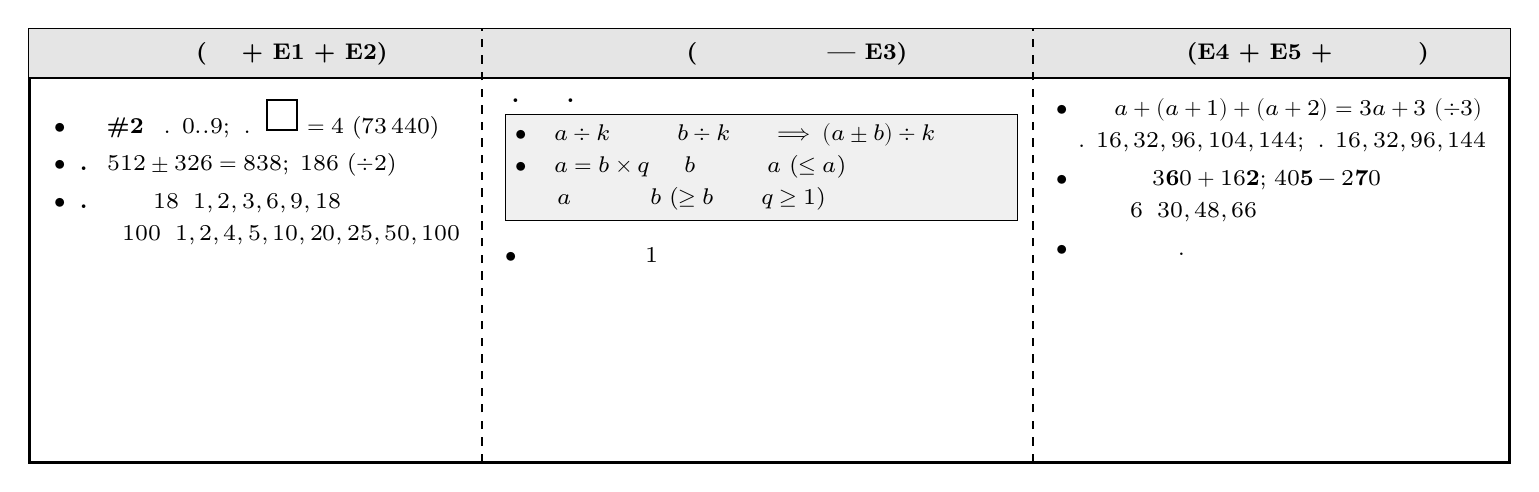
\begin{tikzpicture}[x=1cm, y=1cm, every node/.style={font=\fontsize{8.2pt}{11.6pt}\selectfont, text=black}]
  \draw[black, line width=1.1pt] (0,0) rectangle (18.8,5.50);
  \fill[gray!20] (0,4.88) rectangle (18.8,5.50);
  \draw[black, line width=0.7pt] (0,4.88) -- (18.8,4.88);
  \draw[black, dashed, line width=0.7pt] (5.75,0) -- (5.75,5.50);
  \draw[black, dashed, line width=0.7pt] (12.75,0) -- (12.75,5.50);

  \node at (2.875,5.19) {\textbf{ផ្នែកឆ្វេង (កំណែ + \en{E1} + \en{E2})}};
  \node at (9.25,5.19) {\textbf{ផ្នែកកណ្ដាល (ខ្លឹមសារគោលរក្សាទុក — \en{E3})}};
  \node at (15.775,5.19) {\textbf{ផ្នែកស្ដាំ (\en{E4} + \en{E5} + កិច្ចការផ្ទះ)}};

  % Left
  \node[anchor=north west, text width=5.30cm] at (0.20,4.74) {%
    $\bullet$ \textbf{កំណែ \#2៖} ក. $0..9$; ខ. $\dbox=4$ ($73\,440$)\\[2pt]
    $\bullet$ \textbf{១.២៖} $512\pm 326 = 838;\ 186$ ($\div 2$)\\[2pt]
    $\bullet$ \textbf{២.៖} តួចែកនៃ $18$៖ $1, 2, 3, 6, 9, 18$\\
    \hspace*{0.2cm}តួចែកនៃ $100$៖ $1,2,4,5,10,20,25,50,100$
  };

  % Center
  \node[anchor=north west, text width=6.65cm] at (5.92,4.74) {%
    {\muol\fontsize{8.3pt}{11.8pt}\selectfont ១\enbf{.}២ និង ២\enbf{.} តួចែកនិងពហុគុណ}\\[3pt]
    \tikz\node[draw=black, fill=gray!12, inner sep=3.5pt, text width=6.25cm]{%
      $\bullet$ បើ $a\div k$ ដាច់ និង $b\div k$ ដាច់ $\implies (a\pm b)\div k$ ដាច់\\
      $\bullet$ បើ $a = b\times q$ នោះ $b$ ជា\textbf{តួចែក}នៃ $a$ ($\le a$)\\
      \hspace*{0.2cm}ហើយ $a$ ជា\textbf{ពហុគុណ}នៃ $b$ ($\ge b$ ចំពោះ $q\ge 1$)
    };\\[3.5pt]
    $\bullet$ គ្រប់ចំនួនមានតួចែក $1$ និងខ្លួនឯងជានិច្ច
  };

  % Right
  \node[anchor=north west, text width=5.65cm] at (12.92,4.74) {%
    $\bullet$ \textbf{គំរូ៖} $a+(a+1)+(a+2)=3a+3\ (\div 3)$\\
    \hspace*{0.2cm}ក. $16,32,96,104,144$; ខ. $16,32,96,144$\\[2pt]
    $\bullet$ \textbf{ប្រតិបត្តិ៖} $3\mathbf{6}0+16\mathbf{2}$; $40\mathbf{5}-2\mathbf{7}0$\\
    \hspace*{0.2cm}ពហុគុណនៃ $6$៖ $30, 48, 66$\\[2pt]
    $\bullet$ \textbf{កិច្ចការផ្ទះ៖} ទំ.២៤ លេខ ១ និង លេខ ៣
  };
\end{tikzpicture}
\end{center}

\vfill
\secstrip{២. ចម្លើយផ្ទៀងផ្ទាត់រហ័សសម្រាប់សន្លឹកកិច្ចការសិស្ស \enbf{(}ទំព័រ ១ និង ទំព័រ ២\enbf{)}}{\en{Answer Key}}

\begin{tcolorbox}[
  enhanced, sharp corners, colback=white, colframe=black,
  boxrule=0.8pt, boxsep=2.5pt, top=4pt, bottom=4pt, left=6pt, right=6pt
]
  \fontsize{8.8pt}{13.0pt}\selectfont
  $\bullet$ \textbf{ផ្នែក \en{E1}៖} \textbf{សិស្ស ខ} ត្រឹមត្រូវ ។ \textbf{ផ្នែក \en{E2}៖} \en{E2-A}: $838$ (ដាច់, លេខ $8$), $186$ (ដាច់, លេខ $6$) ។ \en{E2-B}: $18, 9, 6 \to 1,2,3,6,9,18$; $50, 25, 20, 10 \to 1,2,4,5,10,20,25,50,100$ ។\\[2pt]
  $\bullet$ \textbf{ផ្នែក \en{E4}៖} ១) $\mathbf{3a+3}$ ចែកដាច់នឹង $3$ ។ ២) ក. $\mathbf{16, 32, 96, 104, 144}$; ខ. $\mathbf{16, 32, 96, 144}$ ។ \en{EIA}៖ មិនចែកដាច់ទេ!\\[2pt]
  $\bullet$ \textbf{ផ្នែក \en{E5}៖} ១) ក. $3\mathbf{6}0 + 16\mathbf{2}$ (ចម្លើយផ្សេង៖ បើបូកសរុបចែកដាច់នឹង $9$ ដូចជា $310+167=477$ ក៏ត្រូវ ប៉ុន្តែតាមទ្រឹស្ដីបទ ១.២ គឺធ្វើឱ្យតួនីមួយៗចែកដាច់នឹង $9$: $360+162$ និង $405-270$) ។ ខ. (១) $\mathbf{30, 48, 66}$; (២) តួចែកនៃ $15$: $1,3,5,15$; នៃ $24$: $1,2,3,4,6,8,12,24$; នៃ $68$: $1,2,4,17,34,68$; នៃ $120$: $1,2,3,4,5,6,8,10,12,15,20,24,30,40,60,120$ ($16$ ចំនួន) ។ ៣) \textbf{ជម្រើស \en{D}} ។ ៤) សំបុត្រចេញ៖ $\mathbf{1,2,4,5,10,20}$ ។
\end{tcolorbox}

\vfill
\secstrip{៣. ចម្លើយលម្អិតនៃកិច្ចការផ្ទះ \enbf{(}សៀវភៅគោល ទំ.២៤ លេខ ១ និង លេខ ៣\enbf{)}}{សៀវភៅគោល ទំ.២៤}

\begin{tcolorbox}[
  enhanced, sharp corners, colback=white, colframe=black,
  boxrule=0.8pt, boxsep=2.5pt, top=4pt, bottom=4pt, left=6pt, right=6pt
]
  \fontsize{8.7pt}{12.8pt}\selectfont
  $\bullet$ \textbf{លេខ ១ (ទំ.២៤)៖} ក. $78$ និង $120$ គូ ($\div 2$) $\implies 78+120$ ចែកដាច់នឹង $2$ ។ ខ. $4\,140$ ($4+1+4=9\div 3$) និង $720$ ($7+2=9\div 3$) $\implies 4\,140-720$ ចែកដាច់នឹង $3$ ។ គ. $165$ (ចុង $5$) និង $270$ (ចុង $0$) សុទ្ធតែ $\div 5 \implies 165+270$ ចែកដាច់នឹង $5$ ។ ឃ. $5\,130$ ($5+1+3=9$) និង $342$ ($3+4+2=9$) សុទ្ធតែ $\div 9 \implies 5\,130-342$ ចែកដាច់នឹង $9$ ។\\[2pt]
  $\bullet$ \textbf{លេខ ៣ (ទំ.២៤)៖} ចំនួនជាពហុគុណនៃ $30$ ត្រូវបញ្ចប់ដោយលេខ $0$ ($\div 10$) ហើយចែកដាច់នឹង $3$៖ បាន $\mathbf{660}$ ($30\times 22$) និង $\mathbf{540}$ ($30\times 18$) ។ ($645$ ចុង $5$; $610$ ផលបូកខ្ទង់ $7$ មិនចែកដាច់នឹង $3$ ទេ) ។
\end{tcolorbox}

\vfill
\secstrip{៤. ចំណុចប្រុងប្រយ័ត្នគរុកោសល្យសម្រាប់គ្រូ \enbf{(}ការយល់ច្រឡំសំខាន់ៗរបស់សិស្ស\enbf{)}}{\en{Pedagogical Watchlist}}

\begin{tcolorbox}[
  enhanced, sharp corners, colback=panelgray, colframe=black,
  boxrule=0.85pt, boxsep=2.5pt, top=4pt, bottom=4pt, left=6pt, right=6pt
]
  \fontsize{8.6pt}{12.6pt}\selectfont
  $\bullet$ \textbf{តិចនិកចងចាំកុំឱ្យច្រឡំពាក្យ «តួចែក» និង «ពហុគុណ»៖} ណែនាំសិស្សឱ្យភ្ជាប់ពាក្យ \textbf{«ពហុ» = ច្រើនដង (គុណឡើង $\ge n$)} និង \textbf{«តួចែក» = អ្នកយកទៅចែកគេ ($\le n$)} ។\\[2pt]
  $\bullet$ \textbf{ប្រតិបត្តិទំ.១៨ ($3\dbox 0 + 16\dbox$)៖} បើសិស្សបំពេញឱ្យតួនីមួយៗចែកដាច់នឹង $9$ គឺ $3\mathbf{6}0 + 16\mathbf{2}$; បើសិស្សខ្លះបំពេញជា $3\mathbf{1}0 + 16\mathbf{7} = 477$ ($4+7+7=18$) ក៏ផលបូកចែកដាច់នឹង $9$ ដែរ — គ្រូគួរពន្យល់ប្រៀបធៀបវិធីទាំងពីរ!
\end{tcolorbox}

\end{document}
